\documentclass[../poliXuniversity_hospital_(USP)_report.tex]{subfiles}
\graphicspath{ {images/}} 

\begin{document}
\chapter{Motivação}

A dinâmica de hospitais são tão complexas quanto a de fábricas ou industrias. Existem uma rede grande de coolaboradores, fornecedores(remédios,equipamentos e utilitários médicos), controle de estoque(material cirúgico e farmacos), logística de transpote(ambulância) e prestação de serviço(consultas, exames e procedimentos cirúgicos). Se tratando de Hospitais Públicos a otimização desses processos é fator determinante da qualidade do serviço e bom uso dos recursos(limitados) públicos. No HU-USP foi reportado, através do INTEC, a necessidade de tecnolgias que resolvessem três problemas: Contaminação por contato com material laboratoria; Fisioterapia para paciente de mobilidade reduzida e Seleção de medicamentos.

\section{Problemas}

\subsection{Contaminação por contato com amostras laboratorias}

Evideciado pela pandemia, o risco de contaminação por inumeras doenças pelo contato com amostras é algo que ocorre no Hospital Universitario, no qual um colaboradores é designado especificamente ao trabalho de transportar as amostras [FOTO], do ponto de coleta(Pronto Socorro) até o laboratório. O envolvimento de uma terceira pessoa no processo, aquele que transporta o exame, aumenta o risco de espalhamento de patogenos e diminui a segurança sanitária do Hospital

\subsection{Fisioterapia para paciente de mobilidade reduzida}

Com o avanço da pandemia de Covid-19, inumeros pacientes foram internados devido ao processo de entubação ou outras decorrências da doença. Essa imobilização induz perder massa muscular em 48 horas sem o estímulo motor, além de iniciar rápido esse processo se da de forma aguda ao ponto de paciente que passam 1 ou 2 semanas acamados não conseguirem sustentar o peso do próprio corpo. Para resolver isso é necessario um processo de fisio terapia lento, que primeiro depende da recuperação da conciência do paciente para iniciar tratamento, que recupera pouco a pouco a massa muscular, que irá durar semanas. Ou seja, para um paciente reber alta, é necessário que se recupere não só a patologia/lesão que o levou à imobilização como também a perda de massa muscular ocasionada por ela. Quanto mais tempo um paciente permanece na UTI mais gastos por paciente é empregado e menos pacientes são contemplados pelo sistema de Saúde público.

\subsection{Seleção de medicamentos}

Dentro do HU-USP, todos os dias são dedicados 5 horas de trabalho de 4 colaboradores para selecionar os remédios que serão administrados aos pacientes naquele dia. Esses profissionais são enfermeiros ou farmaceûticos que realizam o trabalho mecânico de retirar remédios de gavetas e inserí-los em sacos plasticos [FOTO]. Além de um desperdício de mão de obra qualificada, dado a exaustão do trabalho repetititivo, existe o risco do erro humano na medicação o que pode ser motivo de piora de quadro clinico do paciente ou até óbito. 

\section{Solução proposta}

Após a indentifição desses problemas, a equipe de alunos(ZIMA) com os professores Leopoldo Yoshioka e Oswaldo Horikawa, foram até o hospital universitário[FOTO] à uma visita guiada pelo resposável de cada um dos desafios indenticados. Dr oscar fugita(Diretor do Núcleo de Inovação e Tecnologia (INTEC) e Urologista no Hospital Universitário da USP - SP), Dra. Alexandra siqueira(Coordenadora do Serviço de Fisioterapia no Hospital Universitário da USP) e Dra Valentina Porta(Diretora Técnica da Divisão de Farmácia do HU eProfessora da Faculdade de Ciências Farmacêuticas) guiaram os alunos e explicaram a dinâmica de cada um dos sistemas envolvidos e suas peculiaridades. Com essas informação os alunos, professores e profissionais da saúde chegaram em três conclusões sobre qual abordagem de engenharia usar em cada situação problema. Para a coleta de exames, seria desenvolvido um robô de mobilidade autônoma, para fisioterapia de mobilidade reduzida, um ciclo êrgometro para leitos de UTI e para a seleção de remédios, um selecionador automático de remédios.

\begin{figure}[h]
\centering
    \caption{2° Versão Robô Hospitalar - incompleta}
    \centering % para centralizarmos a figura
    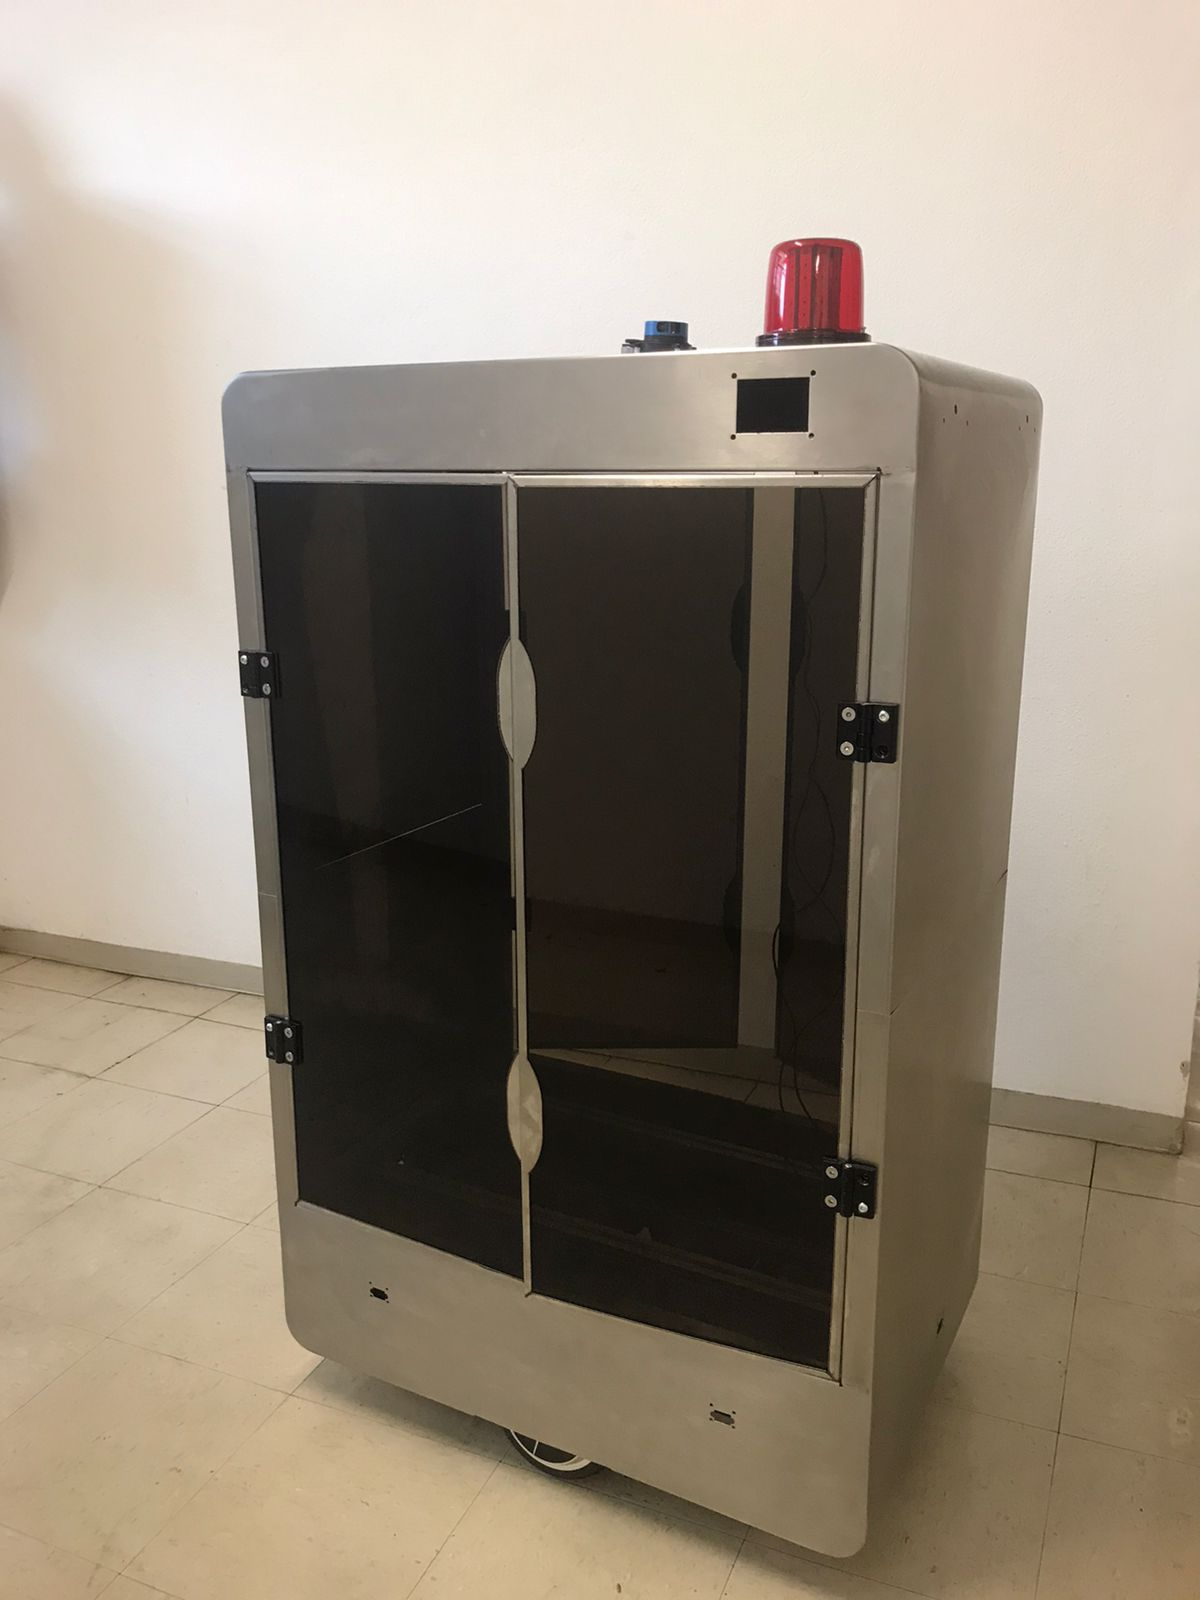
\includegraphics[width=10cm]{v2_robo_hospitalar.jpeg}
    \caption*{Fonte: Escola Politécnica da Universidade de São Paulo}
    \label{figura:1° Versão Robô Hospitalar}
\end{figure}

\end{document}